\chapter{Task Measure Construction}
\label{sec:occclassify}

One step which was skipped over in the informal analysis in the previous chapter was the assignment of occupations into task groups, on the basis of the occupational classification scheme. If task content is to be analyzed rigorously, and in greater detail than a simple three-occupation breakdown, a quantitative view of occupational task content is required. 

\section{Australia \& New Zealand Standard Classification for Occupations (ANZSCO)}

The standard classification scheme for occupations used in Australia, ANZSCO, simply lists by name the tasks a particular job title might be required to perform. These tasks are listed in an occupation-specific way, such that they cannot be compared between occupations. For example, under the unit group 2243: {\em Economists}, the required tasks include
\begin{quote}
{\em Analysing interrelationships between economic variables and studying the effects of government fiscal and monetary policies, expenditure, taxation and other budgetary policies on the economy and the community \citep[p.185]{Trewin2006}}
\end{quote}

{\em Statisticians} (unit group 2441) perform tasks that are largely similar to that of economists, even though the underlying theory that motivates their work may be somewhat different. A corresponding task entry for statisticians includes
\begin{quote}
{\em Defining, analysing and solving complex financial and business problems relating to areas such as insurance premiums, annuities, superannuation funds, pensions and dividends \citep[p.181]{Trewin2006}}
\end{quote}
Given the qualitative nature of this classification scheme, there is no obvious way to systematically formalise the similarity between economists and statisticians on the basis of the ANZSCO classification. However, alternative classification schemes do exist which include comparable task classifications.

\subsection{Occupational tasks: O*NET}\label{sec:onet}

The U.S. equivalent to the ANZSCO classification, the O*NET database, includes hundreds of quantitative scales for the level of work activities, knowledge types and abilities for individuals in each of approximately five hundred occupations. The data were constructed using expert surveys, and provide a very rich source of information about the activities that workers in each occupation actually undertake. For example, for the work activity {\em analyze data}, the occupations {\em economist} and {\em surgeon} score highly (6.58/7 and 5.49/7, respectively.) But for the work activity {\em Handle moving objects}, surgeons score 3.62/7, and economists score only 0.54/7.

We have mapped the ANZSCO (and its predecessors, various editions of ASCO and the CCLO) to the O*NET data, and sucessfully constructued a skill measure series for Australian occupational classification schemes. We then apply a transformation step, described by \citet{Firpo2011}, to build composite indexes for `automation,' `offshorability', and so on. These composite indexes provide a dependent variable which, along with levels of capital investment on an industry-by-industry basis, provide a basis by which changes in the occupational wage structure can be analyzed. The following five composite indexes are constructed for each occupation code:


\begin{enumerate}[A.]
\item Characteristics linked to Technological Change/Offshorability
\begin{enumerate}[1.]
\item Information Content 
  \begin{itemize}
  \item 4.A.1.a.1 Getting Information (JK)
  \item 4.A.2.a.2 Processing Information (JK) 
  \item 4.A.2.a.4 Analyzing Data or Information (JK) 
  \item 4.A.3.b.1 Interacting With Computers (JK) 
  \item 4.A.3.b.6 Documenting/Recording Information (JK)
  \end{itemize}
\item Automation/Routinization 
  \begin{itemize}
  \item 4.C.3.b.2 Degree of Automation 
  \item 4.C.3.b.7 Importance of Repeating Same Tasks 
  \item 4.C.3.b.8 Structured versus Unstructured Work (reverse) 
  \item 4.C.3.d.3 Pace Determined by Speed of Equipment 
  \item 4.C.2.d.1.i Spend Time Making Repetitive Motions
  \end{itemize}
\end{enumerate}
\item Characteristics linked to Non-Offshorability 
\begin{enumerate}[1.]
\item Face-to-Face
\begin{itemize}
  \item 4.C.1.a.2.l Face-to-Face Discussions 
  \item 4.A.4.a.4 Establishing and Maintaining Interpersonal Relationships (JK,B)
  \item 4.A.4.a.5 Assisting and Caring for Others (JK,B) 
  \item 4.A.4.a.8 Performing for or Working Directly with the Public (JK,B) 
  \item 4.A.4.b.5 Coaching and Developing Others (B)
\end{itemize}
\item On-Site Job 
\begin{itemize}
  \item 4.A.1.b.2 Inspecting Equipment, Structures, or Material (JK) 
  \item 4.A.3.a.2 Handling and Moving Objects 
  \item 4.A.3.a.3 Controlling Machines and Processes 
  \item 4.A.3.a.4 Operating Vehicles, Mechanized Devices, or Equipment 
  \item 4.A.3.b.4 Repairing and Maintaining Mechanical Equipment (*0.5) 
  \item 4.A.3.b.5 Repairing and Maintaining Electronic Equipment (*0.5)
\end{itemize}
\item Decision-Making 
\begin{itemize}
\item 4.A.2.b.1 Making Decisions and Solving Problems (JK) 
\item 4.A.2.b.2 Thinking Creatively (JK) 
\item 4.A.2.b.4 Developing Objectives and Strategies 
\item 4.C.1.c.2 Responsibility for Outcomes and Results 
\item 4.C.3.a.2.b Frequency of Decision Making
\end{itemize}
\end{enumerate}
\end{enumerate}

\begin{figure}
  \centering
  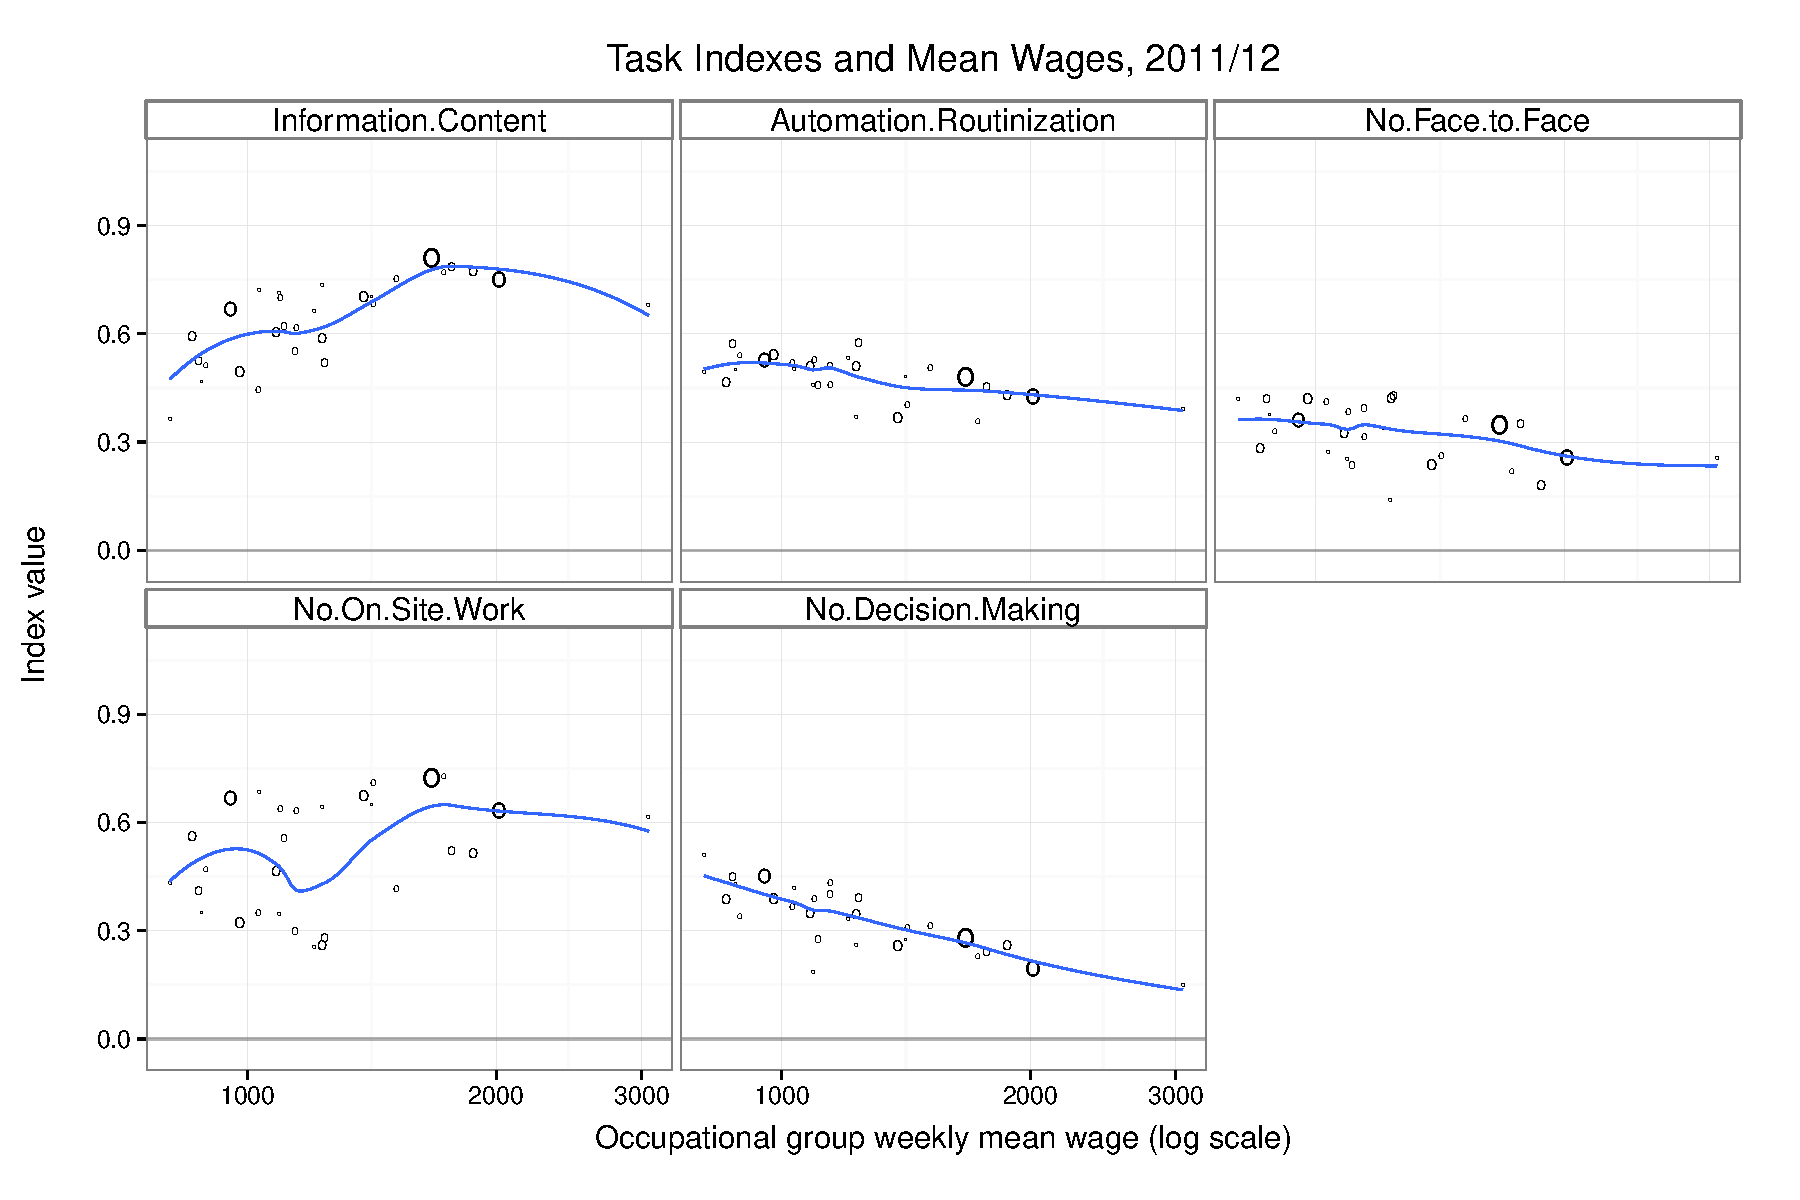
\includegraphics[width=\textwidth]{../figure/wages_indexes.pdf}
  \caption{Mean occupational wage and task measure index values, using second combined grouping. Note the similarity of the observed trend to Figure~\ref{fig:meanocc4dig}, in which occupations have not been grouped. Census respondents reporting full-time work are shown. The loess regression line is weighted by population; circle areas are proportional to population for each occupation. Sources: ABS cat 2072.0, O*NET, US Dept of Labor.}
  \label{fig:meanocc2}
\end{figure}

\begin{figure}
  \centering
  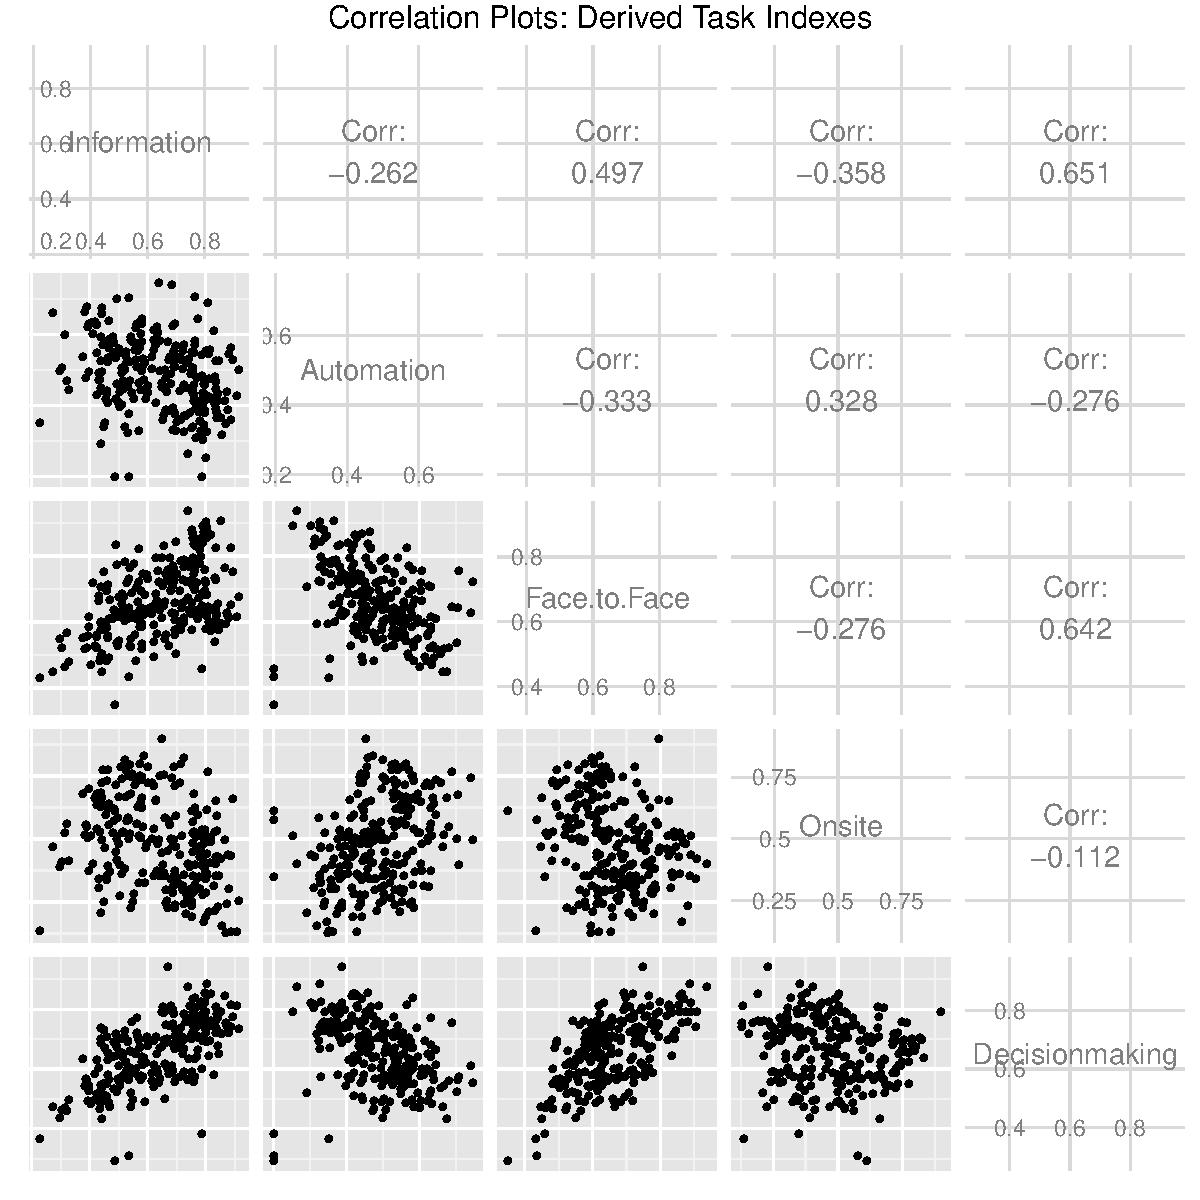
\includegraphics[width=\textwidth]{../figure/correl.pdf}
  \caption{Correlation plots: occupational task indexes for jobs at the ANZSIC 3-digit level. Notice that the job indexes are not perfectly mutually independent. As might be expected, `information content' is positively correlated with `face-to-face' roles ($\rho=0.497$) and decision-making ($\rho=0.651$), but negatively correlated with the job requiring on-site presence ($\rho=-0.358$). `Routinization' is negatively correlated with both face-to-face contact ($\rho=-0.33$) and decision-making ($\rho=-0.276$).}
  \label{fig:correl}
\end{figure}
